\newcommand{\CS}{C\nolinebreak\hspace{-.05em}\raisebox{.6ex}{\bf \#}}

In this section, we present three experiments demonstrating the ease of writing LLM decoding algorithms with semantic constraints for (1) SQL, (2) privacy leakage, and (3) Vega-Lite.
Additionally, \Tool{} implementation supports other languages in our repository, including a large fragment of Python.
\Tool{} code is available at {\color{blue}\url{https://github.com/uiuc-arc/itergen}}

\noindent \textbf{Experimental Setup.}
We run experiments on a 48-core Intel Xeon Silver 4214R CPU with 2 NVidia RTX A5000 GPUs. 
\Tool{} is implemented using PyTorch~\cite{NEURIPS2019_9015}, HuggingFace transformers library~\cite{wolf-etal-2020-transformers} and \syncode{} library~\cite{ugare2024syncodellmgenerationgrammar} for the parser-guided LLM generation infrastructure.


\subsection{SQL Generation}
\label{sec:sql_study}

This case study shows that \Tool{} can improve text to SQL generation. 
Despite providing SQL schema through the prompt, LLM-generated SQL queries can often fail to execute due to mistakes in using accurate table and column names. 
This issue can be easily addressed by selectively resampling column and table names until they exist in the given schema. 
We show that \Tool{} is ideal for implementing a constraint such as this while generating SQL. 
% (See Appendix~\ref{sec:sql_error} for examples)

Figure~\ref{fig:sql_algo} defines a function \str{generate\_sql\_with\_itergen} that utilizes \Tool{} to enhance text-to-SQL generation by ensuring that the generated SQL queries are syntactically accurate and adhere to a specified schema.
The function begins by initializing the generation process with the given prompt and parsing the SQL schema. 
Within a loop, it calls the \str{forward} function, which generates the next output, stopping specifically at either a column name or a table name. 
Here, "column\_name" and "table\_name" are symbols representing non-terminals in our SQL grammar (See Appendix~\ref{sec:sql_grammar} for the full grammar).
The function then checks the validity of this name against the schema using the \str{view} function. 
If the name is invalid, it invokes the \str{backward} function, which moves \Tool{}'s context back to the state before the invalid name was generated, allowing for a new attempt. 
% If a generated column or table name does not match the schema, the function selectively resamples until valid names are produced.
The \str{max\_iter} hyper-parameter prevents infinite looping and excessive computation.

% \ifthenelse{\boolean{iclr}}
% {
% \begin{figure}[htbp]
%     \centering
%     \begin{tcblisting}{
%     listing only, 
%     halign=left,
%     listing engine=minted,
%     minted language=python,
%     minted options={%
%         linenos,
%         breaklines,
%         autogobble,
%         fontsize=\footnotesize,
%         numbersep=2mm,
%         baselinestretch=1},
%     % title=\textbf{\small IterGen code for SQL generation},
%     colbacktitle=blue!30!white, 
%     coltitle=black,
%     left=0pt,               
%     right=0mm,              
%     top=0mm,                
%     bottom=0mm,             
%     boxsep=1mm,
%     width=\textwidth,
%     listing options={style=pythonstyle},
% }
% def generate_sql_with_itergen(iter_gen, problem):
%     iter_gen.start(problem['prompt'])
%     schema = parse_sql_schema(problem)
%     attempts = 0  

%     while not iter_gen.finished() and attempts < max_iter:
%         out = iter_gen.forward(stop_symbols=['column_name', 'table_name'])
%         attempts += 1 

%         if not exists_column(schema, iter_gen.view('column_name')[-1]):
%             iter_gen.backward('column_name')
%             continue

%         if not exists_table(schema, iter_gen.view('table_name')[-1]):
%             iter_gen.backward('table_name')
%             continue

%     return out
% \end{tcblisting}
%     \caption{Code using \Tool{} for LLM-based SQL Generation}
%     \label{fig:sql_algo}
% \end{figure}
% }
% {
\begin{figure}[htbp]
\centering
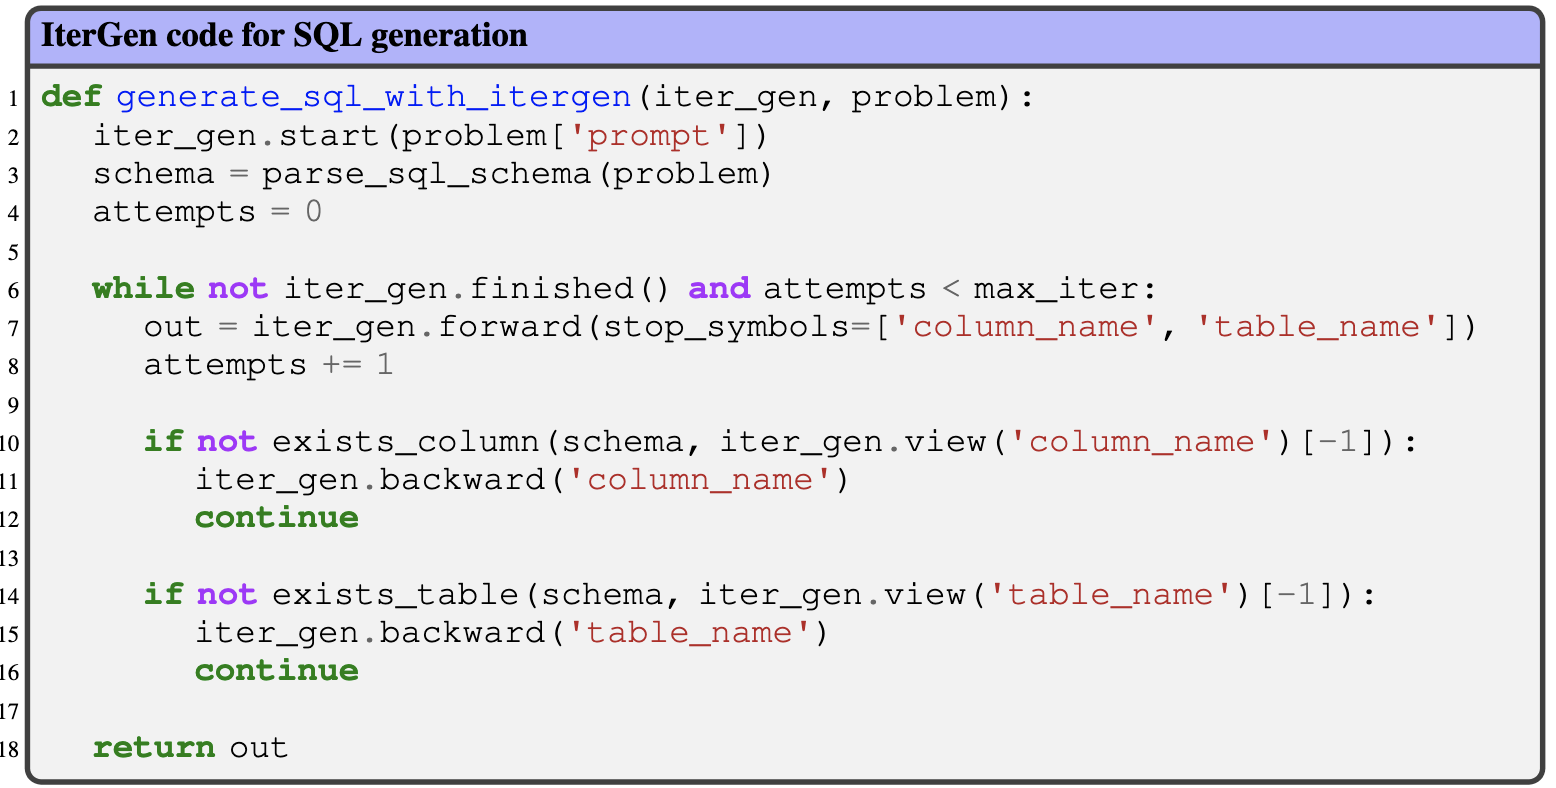
\includegraphics[width=\textwidth]{images/sql_code.png}
\caption{Code using \Tool{} for LLM-based SQL Generation}
\label{fig:sql_algo}
\end{figure}
% }

    

\noindent \textbf{Models.} 
We experiment with a range of state-of-the-art LLMs, including Qwen2.5~\cite{qwen2.5} (base, instruct-tuned, and code-specific) and various models from Llama series~\cite{llamamodels}.

\noindent \textbf{Baselines.}
We use \standard{} unconstrained generation and state-of-the-art grammar-guided generation tool \syncode{}~\cite{ugare2024syncodellmgenerationgrammar} as our baselines. 
\syncode{} will ensure that the LLM-generated SQL queries are syntactically correct, however, it does not guarantee other errors that can occur during the execution of the query.

\noindent \textbf{Datasets.} 
We use the standard Spider~\cite{yu-etal-2018-spider} text-2-SQL dataset for the evaluation.
This dataset has 1034 problems, that are categorized into different difficulty levels - \emph{easy} (250), \emph{medium} (440), \emph{hard} (174), and \emph{extra hard} (170).

We prompt the model with information about the database schema and the text query.
Our prompt is formatted as a user message for instruct-tuned models.
Further, we explicitly prompt the model only to generate the SQL query as it is automatically parsed.
The exact formatting of the prompt is provided in Appendix~\ref{sec:sql_prompt}.
We use greedy decoding for the experiment and set \Tool{}'s maximum limit for moving backward as \str{max\_iter=20} and set the \Tool{} recurrence penalty to 0.7, as it worked well on a small subset of the training dataset. 
We use \str{\textbackslash n\textbackslash n} as an additional stop word to the EOS token for all experiments and use max new token limit as 100 for all three methods. 


\begin{table}[t]
    \scriptsize
    \centering
    \caption{Comparison of \Tool{} and baselines with various models on SQL based on execution accuracy, execution success percentage, number of tokens, and average time.}
    \begin{tabular}{llcccccccc}
        \toprule
        \multirow{2}{*}{\textbf{Model}} & \multirow{2}{*}{\textbf{Method}} & \multicolumn{5}{c}{\textbf{Accuracy (\%)}} & \multirow{2}{*}{\textbf{Execute (\%)}} & \multirow{2}{*}{\textbf{Tokens}} & \multirow{2}{*}{\textbf{Time (s)}} \\
        \cmidrule(lr){3-7}
        & & \textbf{Easy} & \textbf{Medium} & \textbf{Hard} & \textbf{Extra} & \textbf{Overall} & & & \\
        
\midrule

     & \standard{} & 41.6 & 26.8 & 25.9 & 10.0 & 27.5 & 45.8 & 39.30 & 0.607 \\
Qwen2.5-0.5B & \syncode{} & 42.4 & 28.0 & 26.4 & 9.4 & 28.1 & 47.3 & 38.58 & 0.781 \\
\textbf{} & \Tool{} & \textbf{54.8} & \textbf{31.8} & \textbf{33.9} & \textbf{12.4} & \textbf{34.5} & \textbf{60.8} & 40.88 & 0.981 \\

            \midrule
             & \standard{} & 2.8 & 0.2 & 0.6 & 0.6 & 1.0 & 2.3 & 53.27 & 0.827 \\
Qwen2.5-0.5B-Instruct & \syncode{} & 17.2 & 5.9 & 10.3 & 4.7 & 9.2 & 28.3 & 66.79 & 1.525 \\
\textbf{} & \Tool{} & \textbf{36.8} & \textbf{23.4} & \textbf{31.0} & \textbf{11.8} & \textbf{26.0} & \textbf{64.7} & 39.02 & 0.931 \\

            \midrule
             & \standard{} & 70.8 & 47.3 & 37.9 & 27.6 & 48.2 & 78.1 & 35.79 & 0.641 \\
Qwen2.5-1.5B & \syncode{} & 72.0 & 48.0 & 38.5 & 28.2 & 48.9 & 79.0 & 35.48 & 0.810 \\
\textbf{} & \Tool{} & \textbf{73.6} & \textbf{48.4} & \textbf{39.7} & \textbf{28.2} & \textbf{49.7} & \textbf{81.5} & 42.41 & 1.139 \\

            \midrule
             & \standard{} & 0.0 & 0.0 & 0.0 & 0.0 & 0.0 & 0.0 & 44.51 & 0.818 \\
Qwen2.5-1.5B-Instruct & \syncode{} & 43.6 & 29.3 & 33.3 & 24.7 & 32.7 & 60.7 & 54.50 & 1.324 \\
\textbf{} & \Tool{} & \textbf{61.6} & \textbf{47.7} & \textbf{50.0} & \textbf{42.9} & \textbf{50.7} & \textbf{80.0} & 38.44 & 1.015 \\

            \midrule
             & \standard{} & 84.8 & 61.1 & 55.2 & 41.2 & 62.6 & 86.0 & 28.54 & 0.505 \\
Qwen2.5-Coder-1.5B & \syncode{} & 84.8 & 61.1 & 55.2 & 41.2 & 62.6 & 85.6 & 28.74 & 0.620 \\
\textbf{} & \Tool{} & \textbf{84.8} & \textbf{61.6} & \textbf{58.6} & \textbf{43.5} & \textbf{63.7} & \textbf{88.7} & 38.55 & 0.977 \\

            \midrule
             & \standard{} & 40.4 & 24.8 & 20.7 & 10.6 & 25.5 & 50.6 & 37.28 & 0.385 \\
Llama-3.2-1B & \syncode{} & 46.4 & 28.2 & 23.0 & 10.0 & 28.7 & 58.7 & 40.33 & 0.581 \\
\textbf{} & \Tool{} & \textbf{50.4} & \textbf{30.2} & \textbf{23.6} & \textbf{11.8} & \textbf{30.9} & \textbf{67.6} & 38.66 & 0.687 \\

            \midrule
             & \standard{} & 38.0 & 29.5 & 28.2 & 12.4 & 28.5 & 65.3 & 40.42 & 0.714 \\
Llama-3.2-3B & \syncode{} & 46.8 & 34.8 & 32.8 & 19.4 & 34.8 & 78.8 & 39.96 & 0.905 \\
\textbf{} & \Tool{} & \textbf{49.2} & \textbf{35.0} & \textbf{33.3} & \textbf{19.4} & \textbf{35.6} & \textbf{81.4} & 39.08 & 1.042 \\

            \midrule
             & \standard{} & 34.4 & 21.8 & 12.1 & 4.1 & 20.3 & 31.9 & 42.58 & 1.083 \\
Llama-2-7b-chat-hf & \syncode{} & 40.0 & 27.0 & 13.8 & 5.3 & 24.4 & 40.8 & 46.16 & 1.339 \\
\textbf{} & \Tool{} & \textbf{54.0} & \textbf{35.2} & \textbf{27.0} & \textbf{15.3} & \textbf{35.1} & \textbf{64.5} & 51.36 & 1.520 \\

            \midrule
             & \standard{} & 62.0 & 44.3 & 42.0 & 32.4 & 46.2 & 87.7 & 32.95 & 0.895 \\
Meta-Llama-3-8B & \syncode{} & 62.4 & 44.3 & 42.5 & 32.4 & 46.4 & 87.6 & 33.02 & 1.040 \\
\textbf{} & \Tool{} & \textbf{62.8} & \textbf{45.7} & \textbf{43.4} & \textbf{33.5} & \textbf{47.6} & \textbf{89.5} & 32.68 & 1.175 \\

\bottomrule
    \end{tabular}
    \label{tab:sql_comparison}
    \vspace{-.2in}
\end{table}

%%%%%% OLD TABLE BELOW with max_new_tokens=200 problems  %%%%%%%%%%
%  & \standard{} & 41.6 & 26.4 & 25.9 & 10.0 & 27.3 & 45.6 & 56.82 & 0.881 \\
% Qwen2.5-0.5B & \\syncode{}{} & 42.4 & 27.5 & 26.4 & 9.4 & 27.9 & 47.1 & 55.06 & 1.299 \\
% \textbf{} & \Tool{} & \textbf{54.8} & \textbf{31.4} & \textbf{33.9} & \textbf{12.4} & \textbf{34.3} & \textbf{60.6} & 49.19 & 1.231 \\

%             \midrule
%              & \standard{} & 2.8 & 0.2 & 0.6 & 0.6 & 1.0 & 2.3 & 58.65 & 0.883 \\
% Qwen2.5-0.5B-Instruct & \\syncode{}{} & 18.0 & 5.9 & 10.3 & 5.3 & 9.5 & 28.8 & 103.05 & 2.801 \\
% \textbf{} & \Tool{} & \textbf{36.8} & \textbf{23.4} & \textbf{31.0} & \textbf{12.4} & \textbf{26.1} & \textbf{64.8} & 39.69 & 1.046 \\

%             \midrule
%              & \standard{} & 71.2 & 47.3 & 38.5 & 27.6 & 48.4 & 78.6 & 42.37 & 0.747 \\
% Qwen2.5-1.5B & \\syncode{}{} & 72.4 & 48.0 & 39.1 & 28.2 & 49.1 & 79.5 & 42.26 & 1.025 \\
% \textbf{} & \Tool{} & \textbf{73.6} & \textbf{48.6} & \textbf{39.7} & \textbf{28.2} & \textbf{49.8} & \textbf{81.5} & 44.54 & 1.190 \\

%             \midrule
%              & \standard{} & 0.0 & 0.0 & 0.0 & 0.0 & 0.0 & 0.0 & 45.37 & 0.819 \\
% Qwen2.5-1.5B-Instruct & \\syncode{}{} & 43.6 & 29.8 & 33.9 & 25.9 & 33.2 & 61.8 & 74.32 & 2.023 \\
% \textbf{} & \Tool{} & \textbf{61.6} & \textbf{47.7} & \textbf{50.6} & \textbf{42.9} & \textbf{50.8} & \textbf{80.2} & 40.25 & 1.143 \\
 
%         \midrule
%      & \standard{} & 84.8 & 60.9 & 55.2 & 41.8 & 62.6 & 86.4 & 29.82 & 0.530 \\
% Qwen2.5-Coder-1.5B & \\syncode{}{} & 84.8 & 60.9 & 55.2 & 41.8 & 62.6 & 85.9 & 30.59 & 0.679 \\
% \textbf{} & \Tool{} & \textbf{84.8} & \textbf{61.4} & \textbf{58.6} & \textbf{44.1} & \textbf{63.7} & \textbf{88.8} & 39.48 & 1.045 \\

%     \midrule
%      & \standard{} & 40.8 & 24.8 & 20.7 & 10.6 & 25.6 & 51.1 & 48.00 & 0.509 \\
% Llama-3.2-1B & \\syncode{}{} & 46.8 & 28.2 & 23.0 & 10.0 & 28.8 & 59.0 & 56.36 & 0.916 \\
% \textbf{} & \Tool{} & \textbf{50.8} & \textbf{30.2} & \textbf{23.6} & \textbf{11.8} & \textbf{31.0} & \textbf{67.9} & 46.55 & 0.860 \\

%             \midrule
%      & \standard{} & 38.0 & 29.5 & 28.2 & 12.9 & 28.6 & 67.4 & 47.78 & 0.846 \\
% Llama-3.2-3B & \\syncode{}{} & 47.2 & 34.8 & 32.8 & 19.4 & 34.9 & 81.4 & 47.63 & 1.164 \\
% \textbf{} & \Tool{} & \textbf{49.2} & \textbf{35.0} & \textbf{33.3} & \textbf{19.4} & \textbf{35.6} & \textbf{82.1} & 41.73 & 1.163 \\

%     \midrule
%      & \standard{} & 34.4 & 22.0 & 12.1 & 4.1 & 20.4 & 32.6 & 44.74 & 1.148 \\
% Llama-2-7b-chat-hf & \\syncode{}{} & 40.0 & 27.3 & 13.8 & 5.9 & 26.6 & 43.6 & 50.33 & 1.483 \\
% \textbf{} & \Tool{} & \textbf{51.0} & \textbf{35.9} & \textbf{27.0} & \textbf{17.6} & \textbf{35.8} & \textbf{64.9} & 55.12 & 1.833 \\

%             \midrule
%              & \standard{} & 62.0 & 44.3 & 42.0 & 32.4 & 46.2 & 88.5 & 35.11 & 0.961 \\
% Meta-Llama-3-8B & \\syncode{}{} & 62.4 & 44.3 & 42.5 & 32.4 & 46.4 & 88.4 & 35.50 & 1.345 \\
% \textbf{} & \Tool{} & \textbf{63.1} & \textbf{45.7} & \textbf{43.1} & \textbf{33.5} & \textbf{47.6} & \textbf{89.8} & 33.38 & 1.237 \\
% \midrule



%%%%%% OLD TABLE BELOW with 200 problems  %%%%%%%%%%

% \begin{table}[htbp]
%     \scriptsize
%     \centering
%     \begin{tabular}{llccccccc}
%         \toprule
%         \multirow{2}{*}{\textbf{Model}} & \multirow{2}{*}{\textbf{Method}} & \multicolumn{5}{c}{\textbf{Accuracy (\%)}} & \multirow{2}{*}{\textbf{Tokens}} & \multirow{2}{*}{\textbf{Time (s)}} \\
%         \cmidrule(lr){3-7}
%         & & \textbf{Easy} & \textbf{Medium} & \textbf{Hard} & \textbf{Extra} & \textbf{Overall} & & \\
%         \midrule
%         & \standard{} & 61.0 & 23.7 & 10.8 & 0.0 & 24.0 & 43.07 & 1.10 \\
%         Qwen2.5-0.5B & \\syncode{}{} & 61.0 & 26.3 & 10.8 & 0.0 & 25.0 & 44.72 & 1.04 \\
%         & \Tool{} & \textbf{70.7} & \textbf{27.5} & 10.8 & 0.0 & \textbf{27.5} & 44.25 & 1.15 \\
%         \midrule
%          & \standard{} & 0.0 & 0.0 & 0.0 & 0.0 & 0.0 & 60.84 & 0.97 \\
%         Qwen2.5-0.5B-Instruct & \\syncode{}{} & 31.7 & 1.3 & 2.7 & 2.4 & 8.0 & 98.06 & - \\
%         & \Tool{} & \textbf{39.0} & \textbf{26.3} & \textbf{13.5} & \textbf{7.1} & \textbf{22.5} & 45.27 & 1.18 \\
%         \midrule
%          & \standard{} & 85.4 & 33.8 & 27.0 & 11.9 & 38.5 & 38.46 & - \\
%         Qwen2.5-1.5B & \\syncode{}{} & 87.8 & 33.8 & 27.0 & 11.9 & 39.0 & 37.54 & 0.93 \\
%         & \Tool{} & 87.8 & 33.8 & 27.0 & 11.9 & 39.0 & 40.57 & 1.11 \\
%         \midrule
%         & \standard{} & 0.0 & 0.0 & 0.0 & 0.0 & 0.0 & 51.63 & 0.94 \\
%         Qwen2.5-1.5B-Instruct & \\syncode{}{} & 56.1 & 21.2 & 24.3 & 11.9 & 27.0 & 83.9 & - \\
%         & \Tool{} & \textbf{65.9} & \textbf{33.8} & \textbf{40.5} & \textbf{26.2} & \textbf{40.0} & 42.66 & 1.20 \\
%         \midrule
%         & \standard{} & 92.7 & 50.0 & 51.4 & 21.4 & 53.0 & 29.15 & 0.53 \\
%     Qwen2.5-Coder-1.5B & \\syncode{}{} & 92.7 & 50.0 & 51.4 & 21.4 & 53.0 & 29.66 & 0.67 \\
%     & \Tool{} & 92.7 & 50.0 & \textbf{56.8} & 21.4 & \textbf{54.0} & 37.71 & 1.03 \\
%     \midrule
%     & \standard{} & 7.3 & 5.0 & 10.8 & 0.0 & 5.5 & 127.36 & - \\
% Phi-3-mini-instruct & \\syncode{}{} & 43.9 & 30.0 & 27.0 & 14.3 & 29.0 & 69.29 & 2.52 \\
%     & \Tool{} & 43.9 & \textbf{31.2} & \textbf{29.7} & \textbf{26.2} & \textbf{32.5} & 68.41 & 2.72 \\

% CodeLlama-7b-hf & \\syncode{}{} & 51.2 & 45.0 & 27.0 & 14.3 & 36.5 & 51.56 & 1.55 \\
% & \Tool{} & 51.2 & \textbf{46.3} & 27.0 & 14.3 & \textbf{37.0} & 49.40 & 1.67 \\
% \midrule

    
%     \midrule
%      & \standard{} & 34.4 & 22.0 & 12.1 & 4.1 & 20.4 & 32.6 & 44.74 & 1.148 \\
% Llama-2-7b-chat-hf & \\syncode{}{} & 40.0 & 27.3 & 13.8 & 5.9 & 24.6 & 41.6 & 50.33 & 1.483 \\
% \textbf{} & \Tool{} & \textbf{54.0} & \textbf{35.9} & \textbf{27.0} & \textbf{17.6} & \textbf{35.8} & \textbf{66.9} & 55.12 & 1.833 \\

%     \midrule
%      & \standard{} & 27.3 & 20.3 & 19.4 & 6.5 & 19.6 & 78.2 & 48.14 & 1.226 \\
% CodeLlama-7b-hf & \\syncode{}{} & 27.7 & 20.5 & 19.4 & 6.5 & 19.8 & 77.9 & 48.76 & 1.435 \\
% \textbf{} & \Tool{} & \textbf{28.1} & \textbf{21.0} & \textbf{19.4} & \textbf{6.5} & \textbf{20.1} & \textbf{78.2} & 48.24 & 1.640 \\


%     \end{tabular}
%     \caption{Comparison of models on SQL based on accuracy, number of tokens, and average time.}
%     \label{tab:sql_comparison}
% \end{table}

% Present table and results
Table~\ref{tab:sql_comparison} presents our result comparing \standard{} unconstrained generation and \syncode{} to \Tool{}. 
The columns provide insights into each approach's performance: the Accuracy (\%) displays the percentage of correctly generated SQL queries across different difficulty levels, while the Execute (\%) indicates the successful execution percentage of these queries using the SQLite Python interface (execution without runtime errors). 
Additionally, the Tokens column shows the average number of tokens generated, and the Time (s) column reports the average generation time. 
\add{
\Tool{} improves over both baselines with an average overall accuracy of 41.63\% and an execution percentage of 75.84\%, compared to 28.9\% accuracy and 50.28\% execution rate for \standard{} generation. 
It outperforms \syncode{}, which has an average accuracy of 35.22\% and an execution rate of 63.72\%. 
Table~\ref{tab:avg_stats} in Appendix~\ref{tab:avg_stats} presents these averages for each metric over all considered LLMs in the study.
}

We observe that the generation algorithm defined using \Tool{} significantly improves over both baselines for all models in terms of execution accuracy.
For instance, with the Qwen2.5-0.5B model, \Tool{} achieves an overall accuracy of 34.3\%, compared to 27.9\% for the \syncode{}.
Similarly, with the Qwen2.5-1.5B-Instruct model, \Tool{} reaches an overall accuracy of 50.8\%, ahead of \syncode{}'s 33.2\%. 
Our simple \Tool{} written algorithm also substantially reduces the execution errors.  
For Llama-3.2-1B, \Tool{} achieves 67.9\% overall execution success rate, compared to \standard{}'s 51.1\%. 
These results highlight the effectiveness of the \Tool{} approach in generating valid SQL outputs.
We present a detailed comparison of examples where the \Tool{} method avoids the issue in \syncode{} solution in Appendix~\ref{sec:sql_error}.

% \add{
% Furthermore, the \Tool{} approach demonstrates improved time efficiency over \syncode{}. 
% For the Qwen2.5-0.5B model, \Tool{} has an average execution time of 1.23 seconds, slightly faster than \syncode{}'s 1.29 seconds. 
% For Llama-3.2-1B, \Tool{} reduces the average time to 0.86 seconds, outperforming \syncode{}'s 0.91 seconds.
% This is mainly due to the reduced output size in some cases where the model with \Tool{} method halts earlier on generating a valid query, and \standard{} and \syncode{} generate additional redundant tokens. 
% }

Ablation study on recurrence penalty $\gamma$, other modes of prompting with execution feedback, and detailed error analysis is in the Appendix.

% We show some of these examples in Appendix~\ref{sec:sql_error}.

% Overall, \Tool{} improves accuracy by 4\% to 7\% compared to the best-performing syncode, while also boosting execution rates by approximately 10\% to 20\%. 





% \subsection{Privacy Leakage}
% We show that \Tool{} can be successfully applied to drastically reduce total \texttt{leak}ed emails and evaluate on the DecodingTrust ~\cite{wang2023decodingtrust} privacy dataset. To use \Tool{}, we provide a grammar to be followed, defining an \texttt{EMAIL} as a terminal in the grammar. We provide more evaluation details and the code using \Tool{} for reducing privacy leakage in Appendix ~\ref{sec:priv_grammar}. We also show the grammar used for our experiments in Appendix~\ref{sec:priv_grammar}. 


% Note, in our case study, we disallow the exact generation of emails from our corpus. 
% However, \Tool{}s generations may still contain fragments of private email data, due to the simplicity of the email matching function used in the experiment. For more critical applications users may define a more comprehensive matching function. 


% % \noindent \textbf{Baselines.}
% % 
% % We run the base model directly from HuggingFace with no safeguards in place. 
% % \sasa{What does it mean 'standard baseline' ? }




% \noindent \textbf{Datasets.}
% We use 100 problems from the DecodingTrust ~\cite{wang2023decodingtrust} privacy benchmark, focusing on the Enron email extraction setting with the 5-shot prompts specified above. 


% \noindent \textbf{Hyperparameter Values.}
% We use \standard{} unconstrained generation as the baseline. 
% For both the \Tool{} and \standard{} experiments we use greedy sampling. 
% For \Tool{} we set a recurrence penalty \add{$\gamma$ to $0.7$}, and limit the number of per-email backtracking attempts to $10$. 
% % In addition to the models evaluated in~\ref{sec:sql_study}, we further evaluate \Tool{}s privacy preservation ability on the Llama-2-7b, and Llama-3-8B models. 

% Table \ref{tab:model_comparison_1} displays generation metrics of \standard{} generation compared to \Tool{} privacy preserving generation. 
% We display the number of emails leaked by the model in each generation mode, along with the average amount of time spent per generation. 
% Since \Tool{} inherently relies on re-generating certain parts of the completion, we display Average $\Delta$ tokens, a measure of how many more tokens \Tool{} generated on average, per prompt, in comparison to \standard{} generation. 


% We observe a clear, significant improvement over base models, with \Tool{} persevering user privacy with 100\% success. 
% We observe a small increase in average time per completion and average tokens per generation. 
% This overhead consists of mostly discarded tokens when backtracking away from leaky completions, and minor processing delays (e.g., checking for leaks at each step, keeping track of backtracking attempts, moderate fixed overhead when initializing~\Tool{}).
% We also show output perplexity as a response quality gauge to verify that \Tool{}'s secure generations are still providing utility. 
% We notice a marginal increase in response perplexity, indicating a minor divergence from the highest probability tokens, resulting from \Tool{}s replacement of high probability leak-yielding tokens.

% \noindent \textbf{Models.}
% We ran our experiments using the Qwen and $BLANK$ families of models ~\cite{qwen2} (\texttt{Qwen2.5-0.5B-Instruct}, \texttt{Qwen2.5-3B-Instruct}) 

% \begin{table}[h]
%     \centering
%     \caption{Toxicity evaluation for various models}
%     \begin{tabular}{@{}llcccc@{}}
%         \toprule
%         Model                            & Configuration & Avg. Detoxify Score (\%) & Total Tokens & Avg. Runtime (s) \\ \midrule    
%         \multirow{3}{*}{Qwen 2.5 - 0.5B} & Standard       & 2.01      & 10299        & 2.382       \\ 
%                                          & Baseline       & 1.26      & 10402        & 2.398       \\
%                                          & IterGen        & 1.53      &  7139        & 2.76       \\ \midrule
%         \multirow{3}{*}{Qwen 2.5 - 3B}   & Standard       & 5.31      & 11940        & 6.026      \\ 
%                                          & Baseline       & 3.04      & 15033        & 7.503       \\
%                                          & IterGen        & 3.36      &  7877        & 2.395       \\ 
%         \bottomrule
%     \end{tabular}
%     \label{tab:merged_model_metrics}
% \end{table}

% % \begin{table}[htbp]
%     \small
%     \centering
%         \caption{Comparison of models on DecodingTrust based on leakage, number of tokens, and average time.}
%     \label{tab:model_comparison_1}

%     \begin{tabular}{lcccccc}
%         \toprule
%         \multirow{2}{*}{\textbf{Model}} & \multicolumn{2}{c}{\textbf{Leak Rate}} & \multirow{2}{*}{\textbf{Avg. $\Delta$ Tokens}} & \multicolumn{2}{c}{\textbf{Time (s)}} \\
%         \cmidrule(lr){2-3} \cmidrule(lr){5-6}
%         & \textbf{\standard{}} & \textbf{\Tool{}} & & &  \textbf{\standard{}} & \textbf{\Tool{}} \\
%         \midrule
%         Qwen2.5-0.5B-Instruct & 46.0 & 0.0 &  21.7 & 33.69 & 43.4 \\
%         Qwen2.5-1.5B-Instruct & 57.0 & 1.0 &   22.5 & 39.38 & 52.5 \\
%         Phi-3-mini-128k-instruct & 57.0 & 1.0 &  23.11 & 52.9 & 86.75 \\
%         Meta-Llama-3-8B-Instruct & 61.0 & 1.0 &  22.75 & 56.71 & 72.78 \\
%         Llama-2-7b-chat-hf & 59.0 & 0.0 &  24.15 & 52.9 & 65.91 \\
%         Qwen/Qwen2.5-0.5B & 45.0 & 0.0 &  21.14 & 33.98 & 38.19 \\
%         Qwen/Qwen2.5-1.5B & 59.0 & 0.0 &  22.66 & 39.49 & 47.79 \\
%         Meta-Llama-3-8B & 67.0 & 0.0 &   22.93 & 56.19 & 67.15 \\
%         Llama-2-7b-hf & 59.0 & 0.0 & 23.96 & 52.92 & 65.43 \\
%         \bottomrule
%     \end{tabular}
% \end{table}

\begin{table}[htbp]
    \scriptsize
    \centering
        \caption{Comparison of models on DecodingTrust based on leakage, tokens, perplexity, and run time.}
    \label{tab:model_comparison_1}

    \begin{tabular}{lcccccccr}
        \toprule
        \multirow{2}{*}{\textbf{Model}} & \multicolumn{2}{c}{\textbf{Leaks}} & \multicolumn{2}{c}{\textbf{Average Time (s)}} &  \multicolumn{2}{c}{\textbf{Perplexity}} & \multirow{2}{*}{\textbf{Avg.}} \\
        \cmidrule(lr){2-3} \cmidrule(lr){4-5}  \cmidrule(lr){6-7}
        & \textbf{STD} & \textbf{\Tool{}} & \textbf{STD} & \textbf{\Tool{}} & \textbf{STD} & \textbf{\Tool{}} & \textbf{$\Delta$ Tokens} \\
        \midrule
        Qwen2.5-0.5B & 45 & 0 & 0.34 & 0.46 & 6.22 & 6.31 & 4.14 \\

        Qwen2.5-0.5B-Instruct & 46 & 0 & 0.34 & 0.47 & 6.87 & 7.0 & 4.79 \\
        Qwen2.5-1.5B & 59 & 0 & 0.39 & 0.56 & 5.93 & 6.02 & 5.72 \\

        Qwen2.5-1.5B-Instruct & 57 & 0 & 0.39 & 0.58 & 6.17 & 6.28 & 5.95 \\
        Llama-3.2-1B & 62 & 0 & 0.24 & 0.38 & 6.14 & 6.25 & 6.87\\
        Llama-3.2-3B & 61 & 0 & 0.40 & 0.55 & 5.91 & 6.0 & 5.59 \\
        Llama-2-7b-chat-hf & 59 & 0 & 0.53 & 0.66 & 5.97 & 6.07 & 4.15 \\
        Llama-3-8B & 67 & 0 & 0.56 & 0.76 & 5.66 & 5.76 & 7.15 \\
        Llama-3-8B-Instruct & 61 & 0 & 0.57 & 0.78 & 6.18 & 6.30 & 6.02 \\
        \bottomrule
    \end{tabular}
\end{table}

\subsection{Privacy Leakage}
As LLMs continue to proliferate and are integrated into a multitude of applications, it is imperative to protect the private user data used in model pretraining. 
LLMs can inadvertently output data from their training corpus thus exposing private details to end users.
As such, privacy safeguards are critical to mitigate the risks of sensitive information disclosure, (2) further public trust in AI systems, and (3) comply with current and future data protection regulations.   

We evaluate \Tool{} on its capacity to prevent LLMs from ``leaking'' private data to end users. Specifically, a `leak' is defined as an LLM outputting sensitive data that was in its pretraining dataset. While this can happen coincidentally, malicious actors may rely on specifically designed prompts that are intended to make LLMs reveal private data. 
In this case study, we focus on the \emph{Enron} email dataset: a corpus of roughly 600,000 emails between employees of the Enron Corporation. This dataset is often aggregated into large LLM pretraining corpora. As such, most common LLMs have been exposed to this data 
% (including email addresses and message content) 
during their pretraining phase, and thus are capable of leaking the data to end users. 

We show that \Tool{} can be applied to easily prevent private email address leakage. We use the DecodingTrust ~\cite{wang2023decodingtrust} privacy dataset, focusing on the Enron email extraction task. 
We provide an in-depth explanation of the \Tool{} API, as well as experiment details in Appendix ~\ref{sec:privacy_appendix_casestudy}

Table \ref{tab:model_comparison_1} displays generation metrics of \standard{} generation compared to \Tool{} privacy preserving generation. 
We display the number of emails leaked by the model in each generation mode, along with the average amount of time spent per generation. 
Since \Tool{} inherently relies on re-generating certain parts of the completion, we display Average $\Delta$ tokens, a measure of how many more tokens \Tool{} generated on average, per prompt, in comparison to \standard{} generation. 
% \begin{table}[htbp]
%     \small
%     \centering
%         \caption{Comparison of models on DecodingTrust based on leakage, number of tokens, and average time.}
%     \label{tab:model_comparison_1}

%     \begin{tabular}{lcccccc}
%         \toprule
%         \multirow{2}{*}{\textbf{Model}} & \multicolumn{2}{c}{\textbf{Leak Rate}} & \multirow{2}{*}{\textbf{Avg. $\Delta$ Tokens}} & \multicolumn{2}{c}{\textbf{Time (s)}} \\
%         \cmidrule(lr){2-3} \cmidrule(lr){5-6}
%         & \textbf{\standard{}} & \textbf{\Tool{}} & & &  \textbf{\standard{}} & \textbf{\Tool{}} \\
%         \midrule
%         Qwen2.5-0.5B-Instruct & 46.0 & 0.0 &  21.7 & 33.69 & 43.4 \\
%         Qwen2.5-1.5B-Instruct & 57.0 & 1.0 &   22.5 & 39.38 & 52.5 \\
%         Phi-3-mini-128k-instruct & 57.0 & 1.0 &  23.11 & 52.9 & 86.75 \\
%         Meta-Llama-3-8B-Instruct & 61.0 & 1.0 &  22.75 & 56.71 & 72.78 \\
%         Llama-2-7b-chat-hf & 59.0 & 0.0 &  24.15 & 52.9 & 65.91 \\
%         Qwen/Qwen2.5-0.5B & 45.0 & 0.0 &  21.14 & 33.98 & 38.19 \\
%         Qwen/Qwen2.5-1.5B & 59.0 & 0.0 &  22.66 & 39.49 & 47.79 \\
%         Meta-Llama-3-8B & 67.0 & 0.0 &   22.93 & 56.19 & 67.15 \\
%         Llama-2-7b-hf & 59.0 & 0.0 & 23.96 & 52.92 & 65.43 \\
%         \bottomrule
%     \end{tabular}
% \end{table}

\begin{table}[htbp]
    \scriptsize
    \centering
        \caption{Comparison of models on DecodingTrust based on leakage, tokens, perplexity, and run time.}
    \label{tab:model_comparison_1}

    \begin{tabular}{lcccccccr}
        \toprule
        \multirow{2}{*}{\textbf{Model}} & \multicolumn{2}{c}{\textbf{Leaks}} & \multicolumn{2}{c}{\textbf{Average Time (s)}} &  \multicolumn{2}{c}{\textbf{Perplexity}} & \multirow{2}{*}{\textbf{Avg.}} \\
        \cmidrule(lr){2-3} \cmidrule(lr){4-5}  \cmidrule(lr){6-7}
        & \textbf{STD} & \textbf{\Tool{}} & \textbf{STD} & \textbf{\Tool{}} & \textbf{STD} & \textbf{\Tool{}} & \textbf{$\Delta$ Tokens} \\
        \midrule
        Qwen2.5-0.5B & 45 & 0 & 0.34 & 0.46 & 6.22 & 6.31 & 4.14 \\

        Qwen2.5-0.5B-Instruct & 46 & 0 & 0.34 & 0.47 & 6.87 & 7.0 & 4.79 \\
        Qwen2.5-1.5B & 59 & 0 & 0.39 & 0.56 & 5.93 & 6.02 & 5.72 \\

        Qwen2.5-1.5B-Instruct & 57 & 0 & 0.39 & 0.58 & 6.17 & 6.28 & 5.95 \\
        Llama-3.2-1B & 62 & 0 & 0.24 & 0.38 & 6.14 & 6.25 & 6.87\\
        Llama-3.2-3B & 61 & 0 & 0.40 & 0.55 & 5.91 & 6.0 & 5.59 \\
        Llama-2-7b-chat-hf & 59 & 0 & 0.53 & 0.66 & 5.97 & 6.07 & 4.15 \\
        Llama-3-8B & 67 & 0 & 0.56 & 0.76 & 5.66 & 5.76 & 7.15 \\
        Llama-3-8B-Instruct & 61 & 0 & 0.57 & 0.78 & 6.18 & 6.30 & 6.02 \\
        \bottomrule
    \end{tabular}
\end{table}

We observe a clear, significant improvement over base models, with \Tool{} preserving user privacy with 100\% success. 
We observe a small increase in average time per completion and average tokens per generation. 
This overhead consists of mostly discarded tokens when backtracking away from leaky completions and minor processing delays (e.g., checking for leaks at each step, keeping track of backtracking attempts, moderate fixed overhead when initializing~\Tool{}).
We also show output perplexity as a response quality gauge to verify that \Tool{}'s secure generations are still providing utility. 
We notice a small increase in response perplexity, showing a minor divergence from the highest probability tokens, resulting from \Tool{}s replacement of leak-yielding tokens.

\subsection{Vega-lite}
\label{sec:vgl}

\add{
% Explain what vega-lite and NVL corpus is
Vega-Lite~\cite{10.1109/TVCG.2016.2599030} is a declarative language for specifying data visualizations based on a data frame, a tabular structure where rows represent individual data points and columns define attributes of various types. 
Vega-Lite syntax is a subset of JSON, and the Vega-Lite grammar accepts JSON objects conforming to its schema. The detailed grammar for Vega-Lite is provided in Appendix~\ref{sec:vgl_grammar}.
We apply the following constraints with \Tool{}, ensuring precise backtracking before the source of any detected violations:

% \vspace{-0.6}
\begin{itemize}
    \itemsep 1pt 
    \parskip 2pt 
    \item Valid Field Names: Each field name must correspond to a valid column in the data frame.
    \item Field Type Compatibility: The type of each field must follow specific rules. For example, string columns are typically categorical values (nominal in Vega-Lite). If the entries follow ISO timestamp formatting, the column can be interpreted as temporal.
    \item Aggregation Constraints: Aggregations must be limited to specific values, including "count", "mean", "average", and "sum".
\end{itemize}

When checking field type compatibility, we account for the fact that JSON objects are unordered. This means the model may generate either the field name first or the data type first as valid output orders. 
To handle this, we allow the model to complete the generation of the entire object corresponding to the channel, including the field name and the type. 
If a violation is detected, we move backward to the point before the type value. 
% Figure illustrates an example of this process.


\begin{wraptable}{r}{0.62\textwidth}
    \scriptsize
    % \centering
    \vspace{-.2in}
    \caption{Comparing \Tool{} and \syncode{} on the NLV corpus based on accuracy, execution success, and average time.}
    \vspace{-.03in}
    \begin{tabular}{llccc}
        \toprule
        \textbf{Model} & \textbf{Method} & \textbf{Accuracy (\%)} & \textbf{ Execute (\%)} & \textbf{Time (s)} \\
        \midrule
        \multirow{2}{*}{Qwen2.5-1.5B} 
        & \syncode{} & 13.14 & 44.47 & 3.36 \\
        & \Tool{} & \textbf{15.48} & \textbf{46.56} & 3.96 \\
        \midrule
        \multirow{2}{*}{Llama-3.2-3B} 
        & \syncode{} & 31.70 & 85.50 & 4.43 \\
        & \Tool{} & \textbf{36.01} & \textbf{88.21} & 5.00 \\
        \midrule
        \multirow{2}{*}{Llama-3-8B} 
        & \syncode{} & 24.69 & 89.56 & 4.09 \\
        & \Tool{} & \textbf{30.47} & \textbf{92.51} & 4.87 \\
        \bottomrule
    \end{tabular}
    \label{tab:nlv_comparison}
    \vspace{-.2in}
\end{wraptable}



\noindent \textbf{Datasets.}
% Actual evaluation
For the evaluation, we use the NLV Corpus~\cite{Srinivasan_2021}, a dataset comprising 814 examples of text utterances paired with corresponding Vega-Lite visualization specifications.
We use a single-example prompt that explicitly lists all field names from the data frame, as shown in Appendix~\ref{sec:vgl_prompt}.


\noindent \textbf{Hyperparameter Values.}
We use \syncode{}  as the baseline. 
For both \Tool{} and \syncode{} experiments, we use greedy sampling. 
For \Tool{} we set a recurrence penalty \add{$\gamma$ to $0.1$}, and set \str{max\_iter} to 50.
We evaluate three models: Qwen2.5-1.5B, Llama-3.2-3B, and Llama-3-8B. 

% We measure both exact match accuracy to the ground truth and execution success with the Vega-lite compiler.
Table~\ref{tab:nlv_comparison} presents the result for our case study.
The Column "Accuracy" represents the exact match accuracy with the ground truth, the Column "Execute" denotes the execution success with the Vega-lite compiler, and the Column "Time" shows the average time taken for each task.
We observe that the generation algorithm defined using \Tool{} significantly improves over \syncode{} for all models in terms of validation and accuracy.
For instance, with the Llama-3-8B model, \Tool{} achieves an accuracy of 30.5\%, outperforming \syncode{}'s 24.7\%.
Similarly, for the Llama-3.2-3B model, \Tool{} gets an accuracy of 36.0\%, compared to 31.7\% for \syncode{}.
Additionally, \Tool{} demonstrates higher execution rates across all models.
For example, with Qwen2.5-1.5B, \Tool{} achieves an Average Validity of 46.6\%, exceeding \syncode{}'s 44.5\%. We further analyze the evaluation of tasks with Llama-3.2-3B  in the dataset based on the number of iterations and backward calls made by \Tool{} in Figure~\ref{fig:scatter_iters_vs_backwards1} in Appendix~\ref{sec:vgl_appendix_casestudy}.
} 

